\documentclass[11pt, titlepage]{article}
\usepackage{amsmath,amsthm,amssymb}
\usepackage{hyperref, pgf, tikz}
\usepackage{fancyhdr}
\usetikzlibrary{arrows}
\usepackage[margin=1.25in]{geometry}
\usepackage{graphicx}                     
\pagestyle{fancy}
\usepackage{array}
\usepackage{indentfirst}
%\usepackage{wrapfig}

\lhead{Lab \#7}
\rhead{\thepage}
\cfoot{}

\title{Microwave Wavelength and Refraction \\ \ \\ \large Lab \#7}
\author{Name: Avery Karlin \\ Partner: Shantanu Jha}
\date{}
\begin{document}

\maketitle

\begin{center}
\LARGE Microwave Wavelength and Refraction
\end{center}

\section*{Objective}
The objective of the lab is to measure the refraction through a ethafoam prism to find the index of refraction of styrene pellets and the wavelength of the microwave radiation by wave interference.

\section*{Introduction}
Due to the microwave horns being imperfect collectors and transmitters of microwave radiation, in addition to not sending receiving the waves properly aligned, a certain percentage of waves are reflected back to the other side by the horns, forming a standing wave, such that the measurement by the receiver is changed by if they are interfering or multiplying. As a result, if the distance between the transmitter and receiver is $\frac{n\lambda}{2}$.

Refraction is the change in direction of an electromagnetic wave when it crosses the boundary of a medium, called refraction, described by Snell's Law stating $n_1sin(\theta_1) = n_2sin(\theta_2)$, where $\theta$ is the angle between the wave and the normal to the boundary, and n is the medium's index of refraction.

\section*{Procedures and Results}
The receiver and transmitter are first placed such that 1 M is the reading when extremely close together for calibration, moving apart, to some more distant position, finding the maximum reading as the starting point, then moving them closer until 10+ maximums have been seen, measuring the final location as well, such that the wavelength can be calculated by the number of maxima traversed and the distance of traversal. It is then repeated as a second trial, to confirm the results.

Next, the ethafoam prism filled with styrene pellets is placed in the center  such that the side is long foot is perpendicular to the incident beam, finding the angle of the receiver where the signal is the strongest, such that the index of refraction can be calculated. 

\begin{figure}[h]
\centering
\hspace*{0cm}
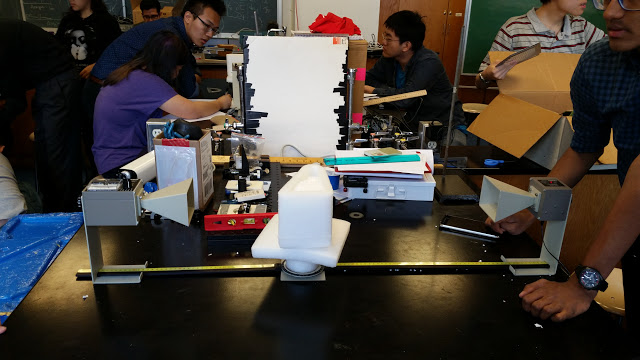
\includegraphics[scale=0.7]{lab71.jpg}
\vspace*{0cm}
\end{figure}

\begin{figure}[h]
\centering
\hspace*{0cm}
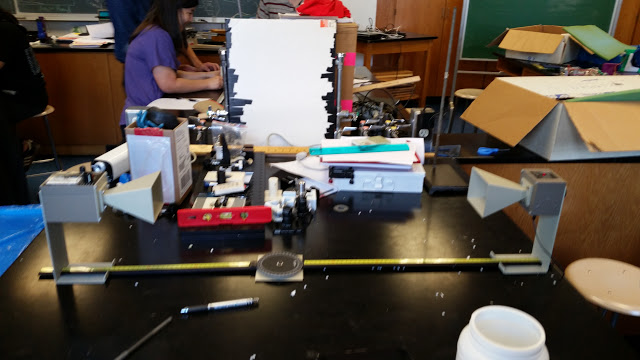
\includegraphics[scale=0.7]{lab72.jpg}
\vspace*{0cm}
\end{figure}

\underline{Wavelength Tests:}
\begin{center}
\begin{tabular}
{|m{7em}|m{7em}|m{7em}|m{7em}|}
\hline
Trial & Initial Position (m) & Maxima Traversed & Final Position (m) \\
\hline
1 & 0.896 & 10 & 0.732 \\
\hline
2 & 0.832 & 10 & 0.585 \\
\hline
\end{tabular}
\end{center}

\underline{Refraction Test:}\\
$\theta = 8^o$\\
$\theta_i = 22^o$\\
$\theta_r = 30^o$

\section*{Discussion}
Calculations for the non-measured data are as shown using the formulas found above:

$$\lambda_1 = \frac{2|\Delta x_1|}{n_1} = \frac{2*|0.732 - 0.896|}{10} = 0.0328 m$$
$$\lambda_2 = \frac{2|\Delta x_2|}{n_2} = \frac{2*|0.585 - 0.832|}{10} = 0.0494 m$$
$$\lambda_{avg} = \frac{\lambda_1 + \lambda_2}{2} = \frac{0.0328 + 0.0494}{2} = 0.0411 m$$
$$f = v\lambda = 3 * 10^8 * 0.0411 = 12.33 GHz$$
$$\text{Percent Error} = \frac{\text{$|$Expected - Actual$|$} * 100\%}{\text{Expected}} =\frac{|12.33 - 10.525| * 100\%}{10.525} = 17.15\%$$
$$n_2 = \frac{sin(\theta_i)n_1}{sin(\theta_r)} = \frac{sin(22^o)*1}{sin(30^o)} = 0.75$$

The error for the frequency could be caused by interference by the air, or the lack of precision at which the waves are reflected by the horns, creating imperfect interference, altering the results. An additional possibility would be the lack of fast enough adjustment of the receiver or lack of precision, compounding to hurt the results.

When the prism is rotated, the intensity changes slightly, such that it must be refracting, since if it was reflected or absorbed, it wouldn't pass through under any orientation, such that it would be unaffected. Rather, since it is refracting, changing the orientation changes how much and the angle by which the waves are refracted, such that the reading would change.

It is not a perfectly valid assumption that the wave is unrefracted when it hits the first side of the prism, due to that assuming it hits straight on by an ideal transmitter, as well as assuming there is no refraction within the air, which would only be true in a vacuum. Thus, it would have to be measured using the same setup, determining if there is any refraction over the distance through the air, by the same test.

It would be expected for the refraction index of the pellets to be slightly lower than that of a pure prism, due to it being less solid, such that it is refracted more randomly, generally back towards the center. In addition, this would likely render the calculations themselves more precise.

\section*{Conclusion}
The average wavelength from the trials of the microwave radiation was 0.0411 m, such that the frequency was 12.33 GHz to the actual value of 10.525 GHz, such that there is a percent error of 17.15\%. It is calculated from the data that the index of refraction of the styrene pellets in the ethafoam prism have an index of refraction of 0.75.

\end{document}
